\documentclass[a4paper,10pt]{article}
%\usepackage[latin1]{inputenc} % Paquetes de idioma (otro encoding)
\usepackage[utf8]{inputenc} % Paquetes de idioma
\usepackage[spanish]{babel} % Paquetes de idioma
\usepackage{graphicx} % Paquete para ingresar gráficos
\usepackage{grffile}
\usepackage{hyperref}
\usepackage{fancybox}
\usepackage{amsmath}
\usepackage{amsfonts}
\usepackage{listings}
% Paquetes de macros de Circuitos
%\usepackage{pstricks}
\usepackage{tikz}

% Encabezado y Pié de página
\usepackage{fancyhdr} % Paquete para encabezados y pie de página
\pagestyle{fancy} % Sin esta línea no se imprimiría el encabezado en todas las páginas

\fancyhf{} %  Borra el encabezado anterior (Por defecto escribe el títutlo de la sección en la que se encuentra la hoja
\setlength{\headheight}{22.55pt}
\fancyhead[L]{
	{\textsf{Facultad de Ingenier\'ia $-$ Universidad de Buenos Aires \\ 66.09 Laboratorio de Microcomputadoras}}
}
%\addtocounter{page}{5}
\fancyhead[R]{\thepage}

\renewcommand{\footrulewidth}{0.4pt} % Ajusta el tamaño de las líneas separadoras en el pié de página
\renewcommand{\headrulewidth}{0.4pt} % Ajusta el tamaño de las líneas separadoras en el encabezado

\fancyfoot[L]{
	{\textsf{Anteproyecto} \\
	{\textsf{Integrantes: Torres Feyuk, Levi Hadid}}
	}
}
		

% Carátula del Trabajo
\title{ \author{} % Lo pongo para que el warning no moleste :p
\setlength{\unitlength}{1cm} %  Especifica la unidad de trabajo
\thispagestyle{empty}

\begin{picture}(18,0)
\put(0,0){
\includegraphics[width=1.5cm, height=3cm]{Imagenes/Logo1.png}}

\put(10.5,0){
\includegraphics[width=3cm, height=3cm]{Imagenes/Logo2.png}}

\end{picture}
\\[1.5cm]
\begin{center}
	\textbf{{\Huge Facultad de Ingenier\'ia \\ Universidad de Buenos Aires}}\\[2cm]
	{66.09 Laboratorio de Microcomputadoras}\\[0.5cm]
	{Anteproyecto}\\[2.5cm]
\end{center}

\begin{flushleft}
	\textbf{Integrantes:} \\[1cm]

	\begin{tabular}{|c|c|c|}
		\hline
		\textbf{\normalsize Padr\'on} & \textbf{\normalsize Nombre} & \textbf{\normalsize Email} \\
		\hline
		\normalsize 89579 & \normalsize Torres Feyuk, Nicol\'as R. Ezequiel & \normalsize ezequiel.torresfeyuk@gmail.com \\
		\hline
		\normalsize 90406 & \normalsize Levi Hadid, Lucas Alberto & \normalsize lucaslh9@hotmail.com \\
%		\hline
%		\normalsize ????? & \normalsize Madariaga, Eduardo & \normalsize madariagaedu@gmail.com \\
		\hline
	\end{tabular}
\end{flushleft}
\date{} % Hace que no se imprima la fecha en la cual se compilo el .tex
 }

\begin{document}
	\maketitle % Hace que el título anterior sea el principal del documento
	\newpage

	\tableofcontents % Esta línea genera un indice a partir de las secciones y subsecciones creadas en el documento
	\newpage

	\section{Objetivos}
		El objetivo del presente trabajo práctico consiste en diseñar e implementar un sistema que permita controlar los motores de un autito RC mediante 
		comunicación inalámbrica. 

	\section{Prestaciones Técnicas}
		\begin{itemize}
			\item El autito debe contar con 4 velocidades de funcionamiento, algo similar a una caja de cambios.
			\item La comunicación inalámbrica debe abarcar un rango máximo de 10 metros. 
			\item Se debe tener un control absoluto del auto a través del control remoto
			\item Se debe alimentar tanto a la plaqueta del control como la del auto con baterias de 9V.
		\end{itemize} 

	\section{Descripción del Proyecto}
		El proyecto consiste en realizar el sistema de control de un auto de juguete el cual utiliza motores de continua para desplazarse, de forma tal de 
		manejar al mismo de forma remota a través de un control. Dado que lo que se desea es diseñar y construir el sistema y no la parte mecánica, se
		 utiliza en el presente proyecto  el chasis y los motores de un autito de juguete. \\
		\indent El vehículo a utilizar consta de dos motores de continua en las ruedas traseras del mismo. De esta forma, para lograr que el vehículo gire 
		tanto a la derecha como a la izquierda se debe alimentar a uno de los motores mientras el otro se mantiene fijo. Para lograr que el auto se desplace 
		para adelante o atrás solo basta con alimentar a los motores con la misma señal de forma que se muevan para el mismo lado y con la misma 
		potencia. \\
		\indent El auto será controlado a través de un control remoto que se encontrará enviando constantemente una señal al autito. Este último procesará 
		esta señal
		y según lo recibido se moverá en la dirección indicada y cambiará su velocidad a la indicada.
	
		
	\section{Diagramas en Bloques}
		\subsection{Autito}
			En la figura \ref{timg004} se exhibe el diagrama en bloques del autito. El mismo es muy sencillo pero básicamente es el corazón del TP dado que 
			muestra como a partir del puente H se van a controlar los motores del autito. 
			\begin{figure}[!htb]
				\centering
				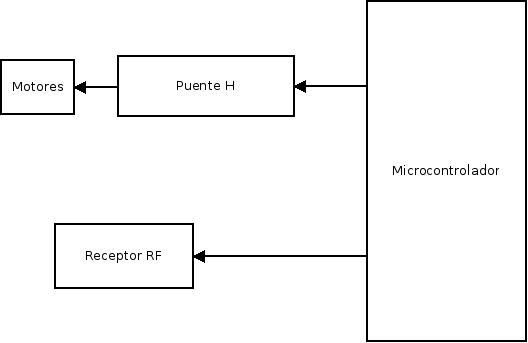
\includegraphics[width=9cm]{Imagenes/DiaBloqAutito.jpg}
				\caption{Diagrama en Bloques del Autito} \label{timg004}
			\end{figure}
		\subsection{Control}
			En la figura \ref{limg001} se exhibe el diagrama en bloques del control remoto. Este diagrama posee más bloques funcionales dado que los 
			agregados que posee el proyecto como lo es el manejo de velocidades se controla en esta plaqueta.  
			\begin{figure}[!htb]
				\centering
				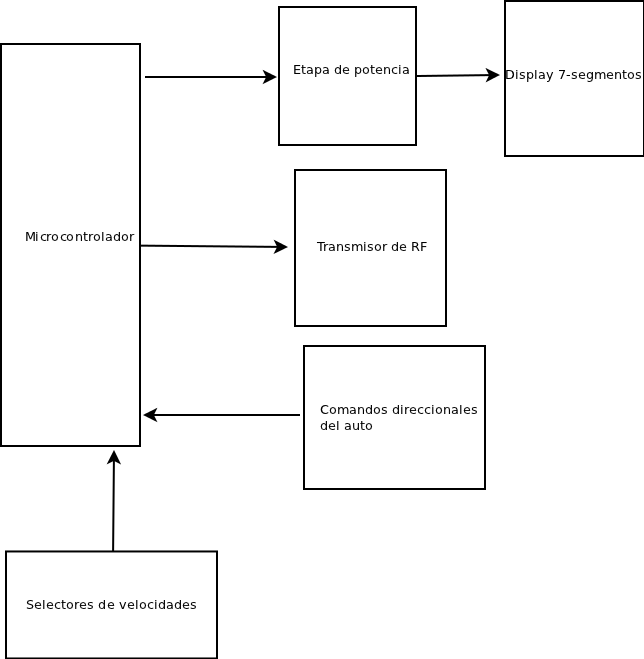
\includegraphics[width=9cm]{Imagenes/Diagrama1.png}
				\caption{Diagrama en Bloques del Control} \label{limg001}
			\end{figure}

	\section{Circuitos Esquemáticos}
		\subsection{Autito}
			En la figura \ref{timg001} se exhibe el circuito esquemático de la plaqueta del autito. A continuación se procede a explicar los componentes más 
			importantes del circuito diseñado.

			\begin{figure}[!htb]
				\centering
				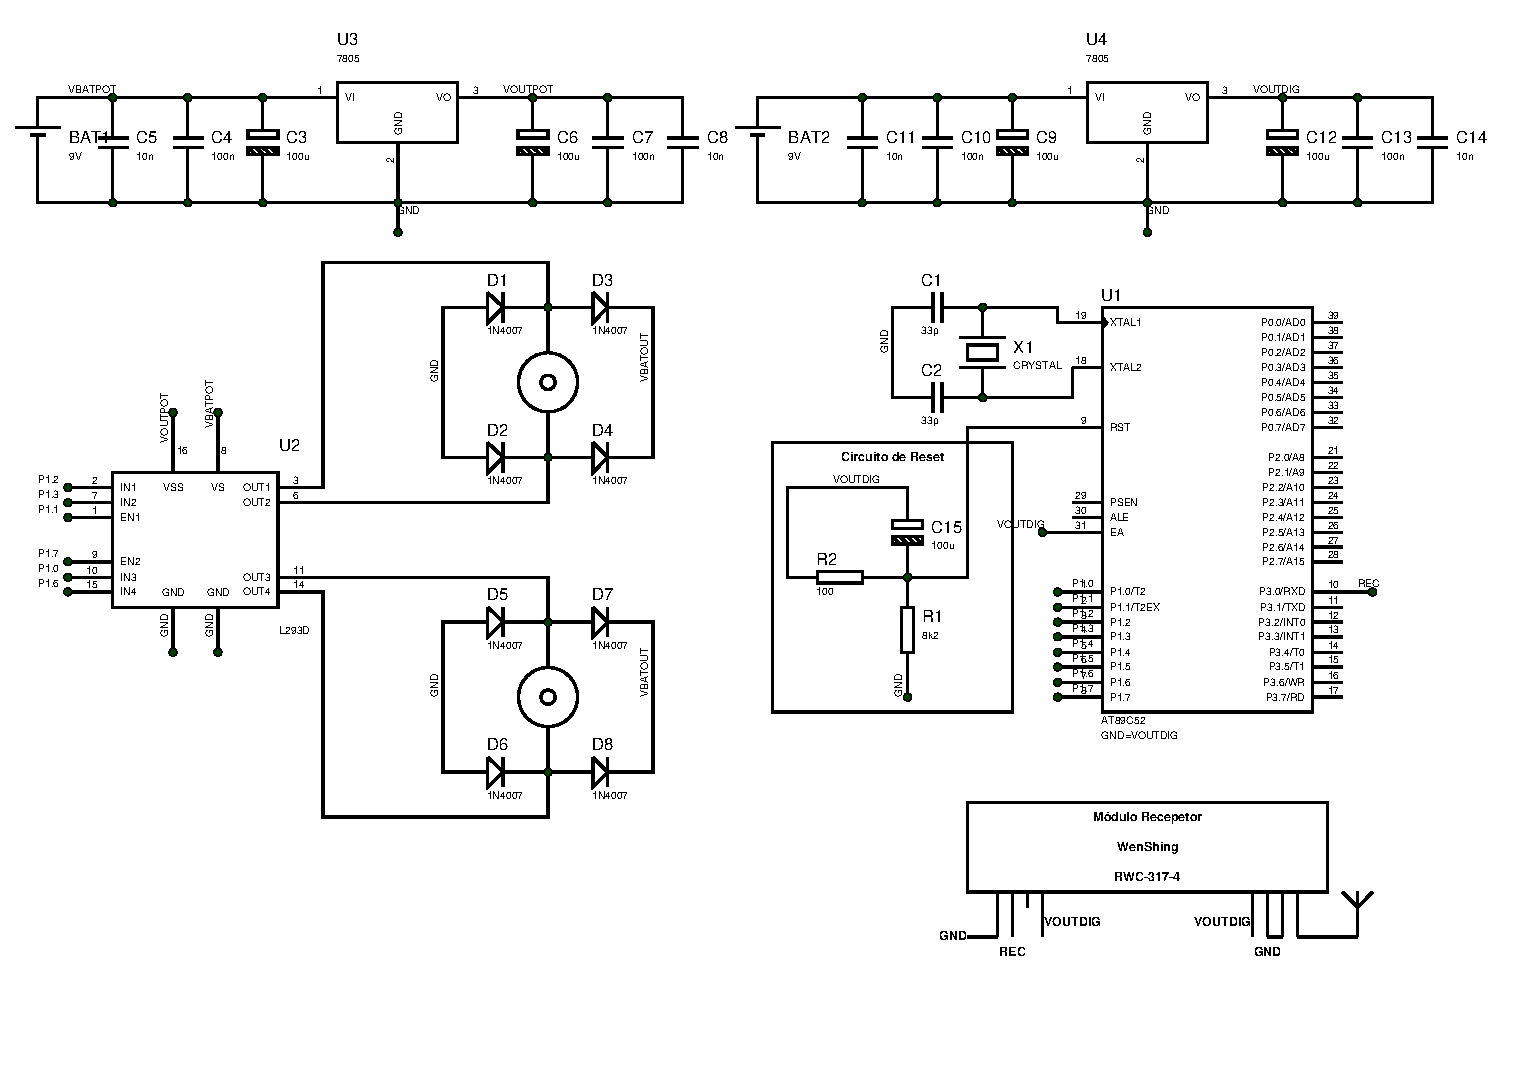
\includegraphics[width=14cm]{Imagenes/EsquematicoAuto.PDF}
				\caption{Esquemático de la plaqueta del Autito} \label{timg001}
			\end{figure}

				\subsubsection{Parte Analógica y Parte Digital}
					Debido a que los motores del vehículo introducen ruido que afecta el funcionamiento de otros integrados (como puede ser el micro), se hizo una 
					separación entre la parte digital del circuito y la parte analógica. La separación se realiza de dos formas: 
			
					\begin{itemize}
						\item Primero, se utilizaron fuentes diferentes para alimentar a estas dos etapas. Esto se debe a que la etapa de potencia analógica consume
						mucha más potencia que la parte digital, debido a que esta es la que se encarga de proveerle la energía necesaria a los motores para que 
						estos funcionen.
						\item Segundo, se diseña la placa forma que la tierra de estas dos etapas bien definidas se encuentren desacopladas. Esto mismo se puede observar
						en la figura \ref{timg002} donde se exhibe el PCB del autito. Las dos tierras, tanto la digital como la analógica se unen en un sólo punto en el 
						cual se conectan además las baterias del autito. Con este conexionado, el ruido que pueda llegar a generarse en la etapa de analógica no llega a 
						la etapa digital.    
					\end{itemize}

					\begin{figure}[!htb]
						\centering
						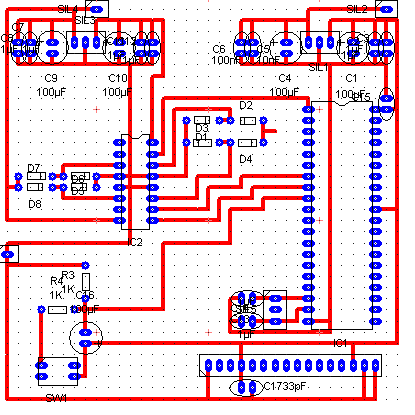
\includegraphics[width=9cm]{Imagenes/PCBAutito.png}
						\caption{PCB de la plaqueta del autito} \label{timg002}
					\end{figure}


				\subsubsection{Motores}
					Los motores utilizados en el vehículo, como se ha mencionado anteriormente, son motores de continua. Los mismos funcionan haciendo girar 
					al mismo en función del valor medio de la señal que se inserte entre sus terminales. Si el valor medio de la señal ingresada es positiva, el mismo 
					girará para un lado mientras que si la misma es  negativa el motor girará para el lado contrario. \\
					\indent	El microncontrolador sólo puede manejar los estados lógicos 0 y 1 a través de sus puertos. El estado 1 es representado por una tensión de 
					5$~\text{V}$ y el estado 0 es representado por una tensión de $0~\text{V}$. Si bien los estados en realidad están asociados a un rango de valores 
					válidos más que a un valor fijo, lo importante es que en ninguno de estos estados el micro puede entregar una tensión negativa.
					\indent Para solucionar este problema se utiliza un circuito muy conocido llamado \emph{Puente H}. El mismo se utiliza para a través de 
					señales que no poseen la particularidad de alternar entre polaridad positiva y negativa poder controlar la dirección de giro de un motor. Debido a 
					lo conocido de este circuito, el mismo se puede comprar como circuito integrado. El integrado utilizado en el presente proyecto es el 
					\emph{L293D}. El diagrama del mismo se exhibe en la figura \ref{timg003}.	  

					\begin{figure}[!htb]
						\centering
						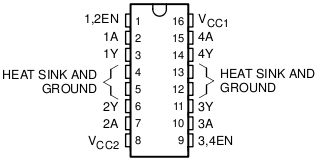
\includegraphics[width=7cm]{Imagenes/puenteH.jpg}
						\caption{Esquemático de la plaqueta del Control} \label{timg003}
					\end{figure}

					El integrado L293D contiene 2 puentes H, uno de cada lado de la pastilla del integrado. Los pines de salida Y son los que van conectados a 
					los terminales del motor. A partir de las entradas A y EN se controla el funcionamiento del mismo. En la tabla \ref{tab001} se exhibe como 
					conectar a los mismos para poder controlar correctamente los motores.
				
					\begin{table}[!htp]
						\centering
						\begin{tabular}{|c|c|c|c|}
							\hline
							1,2EN & 1A & 2A & Función \\
							\hline
							H & L & L & Motor Frenado \\
							\hline 
							H & L	& H & Girar a la Derecha \\
							\hline
							H & H & L & Girar a la Izquierda \\
							\hline
							H & H & H &  Motor Frenado \\
							\hline
							L & X & X & Motor Libre \\	
							\hline
						\end{tabular}
					\caption{Tabla de Resultados} \label{tab001}
					\end{table}

					En el circuito esquemático de la figura \ref{timg001} se puede observar que el microcontrolador maneja los motores a través del puerto 1. El puerto 1 
					como se sabe posee resistencias de pull-up, de forma que se conecta directamente las salidas del puerto a las entradas del integrado L293D. En el caso
					de este integrado, no fue necesario agregar una etapa de potencia entre el micro y el puente H dado que las corrientes que exije el L293D menores a las
					máximas que puede soportar los pines del puerto (100 uA máximos del L293D contra aproximadamente 10 mA máximos que soporta cada pin del 
					microntrolador). \\
					\indent Para comandar los motores se utiliza la entrada de habilitación EN que provee el integrado \emph{L293D}. A la entrada de potencia
					VS se conecta directamente la alimentación de la batería.  De esta forma, a partir de la señal ingresada en VEN se regula el valor medio de la 
					señal que le llega a los motores. El microcontrolador se encarga de generar señales cuadradas que, según el duty cycle de las mismas, 
					cambia el valor medio de la continua que le llega a los motores. \\
					\indent Los motores poseen diodos conectados entre sus terminales, para prevenir el paso de corrientes inversas al integrado de potencia y evitar
					que el mismo se queme. 

				\subsubsection{Comunicación Inalámbrica}	
			 		La comunicación entre el control y el autito se realiza por medio de transmisión serie. Esto se realiza gracias a que los microcontroladores de
					la familia 8051 poseen un puerto serie integrado en el mismo. Se utiliza al puerto serie como una UART de 8 bits para enviar y recibir datos entre 
					el autito y el control . \\
					\indent Sin embargo, dado que como se 
					expuso en las prestaciones técnicas la comunicación entre el control y el auto debe ser inalámbrica, se utilizan en el presente proyecto un par
					de módulos apareados que se encargan de resolver este problema. Estos módulos son el TWS-BS3 (Transmisor) y el RWS-317-4 (Receptor). Los
					mismos envían y reciben información de forma serie modulando la señal en AM a una frecuencia de 433.12$~\text{MHz}$. Dado que los mismos trasmiten
					de forma serie, basta con conectar directamente el pin de recepción de \emph{data} del receptor a la entrada \emph{RXD} del microcontrolador del 
					autito para recibir la información enviada por el control. 
				
		\subsection{Control}
			La placa de control es alimentada con una batería de 9V. Se utiliza el
			dispositivo 7805 para adaptar la tensión de 9V entregada por la batería
			a una tensión de 5V necesaria para el funcionamiento del microcontrolador (AT89S52).
			El 7805 se inserta en el circuito acompañado de una configuración de capacitores de
			100uF, 100nF y 10nF, como puede observarse en la figura \ref{limg002}. Estos capacitores cumplen la función de estabilizar la tensión de 
			alimentación en VCC=5V para que no haya oscilaciones indeseables de tensión respecto del valor requerido.
			La pata de VCC del microcontrolador AT89S52 es conectada a los 5V obtenidos de la pata de VCC de salida del 7805, y de esta forma se alimenta al 
			microcontrolador. También se conecta la pata EA del microcontrolador a VCC para que el micro utilice la ROM interna para código. Entre los terminales 
			XTAL1 y XTAL2 se conecta un cristal de 11.059MHz de la forma en que se muestra en la figura \ref{limg002}. \\
			\indent En la figura podemos ver también el circuito de reset utilizado. Este se conecta a la pata RST del microcontrolador y consta de una 
			resistencia de 100$\Omega$, una de 8.2k$\Omega$, un capacitor de 100uF y un pulsador. Al apretar el pulsador, la pata RST del micro se pone en estado 
			alto hasta que éste deje de ser pulsado. El capacitor hace que se mantenga en estado alto esta pata durante el tiempo necesario para que el micro se 
			termine de resetar. Este tiempo depende exclusivamente de lo que tarde en estabilizarse el oscilador utilizado por el microcontrolador. Por lo general,
			el tiempo que tardan los mismos en estabilizarse es del orden de los milisegundos, de ahí que el \emph{Tau} del circuito de reset compuesto por el 
			capacitor de 10 uF y la resistencia de $8.2~\text{k}\Omega$ sea de 82 ms. \\   
			\indent Todos los puertos del microcontrolador, a excepción del puerto 0, tienen una red de pull-up que permite trabajar con estos puertos 
			sin necesidad de utilizar una alimentación externa (ya que internamente, cada uno de los pines del puerto está conectado a VCC a través de una 
			resistencia de pull-up).\\
			\indent Se utilizó el puerto 2, más especificamente las patas P2.0, P2.1, P2.2 y P2.3, como los terminales del microcontrolador a través de 
			los cuales se ingresan los de comandos de dirección que controlarán el autito. Estos comandos son ingresados al micro a través de 4 pulsadores, 
			uno para cada dirección (adelante, atrás, izquierda, derecha). Cada véz que se presionan los pulsadores, se conecta las correspondientes patas del 
			puerto a GND, lo que hace que se escriba un 0 en éstas. De esta forma, el micro actuará de la forma adecuada en concordancia con la entrada 
			ingresada. \\
			\indent A las patas de interrupciones INT0 e INT1 se conectan 2 pulsadores que se utilizarán para cambiar las velocidades. Estos pulsadores son 
			conectados de la misma forma que aquellos que controlan las direcciones del autito.\\
			\indent El puerto 1 se utiliza para controlar un display 7-segmentos que se encarga de mostrar la velocidad a la que está funcionando el autito. 
			Como el puerto es incapaz de entregar la potencia necesaria para hacer funcionar correctamente el display de 7-segmentos, se conecta como etapa 
			intermedia entre el microcontrolador y el display, una etapa de potencia proporcionada por el dispositivo ULN2803, qué basicamente es un array 
			de transistores que se encarga de aumentar la corriente entrante al display (corriente que el microcontrolador es incapaz de entregar por sí solo). \\
			\indent En la figura \ref{limg002} se puede ver la forma de conexionado entre el microcontrolador, el ULN2803, y el display 7-segmentos. El ULN2803 
			tiene varias entradas y salidas (una entrada-salida para cada pata del puerto correspondiente con cada led) y una pata de GND que se conecta a la 
			masa del circuito. Entre el ULN2803 y el display,se colocaron, en cada una de las lineas correspondientes a cada led del display, resistencias de 
			270$\Omega$ para limitar la corriente que circula por cada led y evitar,de esta forma, que los mismos se quemen. Las patas del puerto del micro se
			conectan a las entradas del ULN2803, como puede verse en la fugra \ref{limg002}. Se agregaron resistencias de 2.7k$\Omega$ entre las patas del puerto 
			y VCC de manera tal de generar una resistencia de pull-up equivalente menor (resultado del paralelo entre la resistencia de pull-up interna del micro 
			y la resistencia agregada), que le permita al micro entregar una mayor corriente necesaria para alimentar al ULN2803, y conseguir de esta forma el 
			correcto funcionamiento del display 7-segmentos. \\
			\indent Para la transmisión RF, se uso el módulo TWS-BS3. Este módulo cuenta con 4 patas: una que se conecta a VCC, otra que se conecta a GND, otra 
			que recibe la información digital proveniente del puerto serie del micro, más específicamente de la pata TXD, y una última pata que es la que se 
			conecta a la antena necesaria para transmitir.\\
			
			\begin{figure}[!htb]
				\centering
				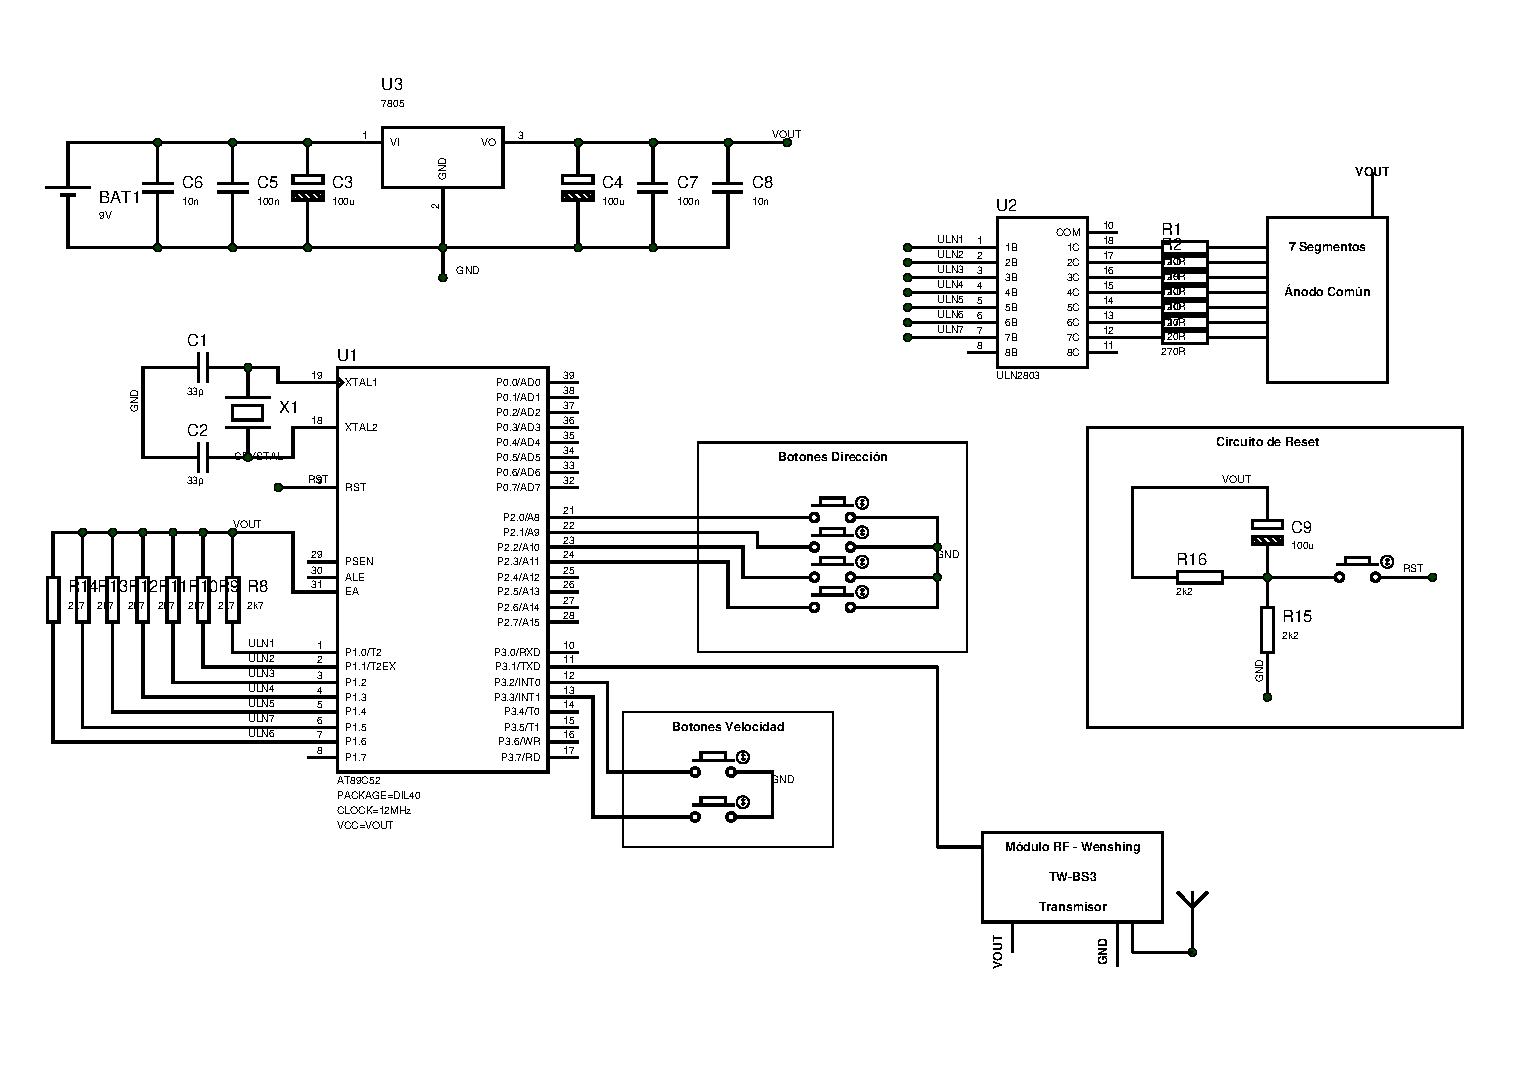
\includegraphics[width=14cm]{Imagenes/EsquematicoControl.PDF}
				\caption{Esquemático de la plaqueta del Control} \label{limg002}
			\end{figure}
	
	\section{Listado de Componentes}
	
		\begin{tabular}{|c|c|c|}
			\hline
			\textbf{Componente} & \textbf{Precio Unit. (U\$S}) & \textbf{Cantidad} \\
			\hline
			Placas experimentales 10cm X 10cm & 4.08 & 2\\
			\hline
			Placas experimentales 10cm X 5cm & 2.14 & 1\\
			\hline
			Baterías de 9V & 4.16 & 3\\
			\hline
			AT89S52 & 2.80 & 2\\
			\hline
			TWS-BS3 & 4.74 & 1\\
			\hline
			RWS-371-4 & 4.74 & 1\\
			\hline
			Regulador 7805 & 0.420 & 3\\
			\hline
			L293D (Puente H) & 4.10 & 1\\
			\hline
			ULN2803 & 0.68 & 1\\
			\hline
			Cristales 11.059MHz & 0.36 & 2\\
			\hline
			Diodos & 0.02 & 8\\
			\hline
			Pulsadores & 0.10 & 8\\
			\hline
			Capacitores 33 pF & 0.04 & 5\\
			\hline
			Capacitores 10 nF & 0.04 & 8\\
			\hline
			Capacitores 100 nF & 0.04 & 7\\
			\hline
			Capacitores 10 uF & 0.03 & 2\\
			\hline
			Capacitores 100 uF & 0.03 & 7\\
			\hline
			Resistencias 100$\Omega$ & 0.014 & 2\\
			\hline
			Resistencias 270$\Omega$ - 5\% & 0.014& 7\\
			\hline
			Resistencias 2.7k$\Omega$ - 5\% & 0.014 & 7\\
			\hline
			Resistencias 8.2k$\Omega$ - 5\% & 0.014 & 2\\
			\hline
			Zócalos - 40 patas & 0.14 & 2\\
			\hline
			Zócalos - 9 patas & 0.07 & 1\\
			\hline
			Zócalos - 8 patas & 0.06 & 1\\
			\hline
			Motores DC & 21.04 & 2\\
			\hline
			\hline
			\textbf{Total} & \multicolumn{2}{|c|}{\textbf{U\$S 89.46}} \\
			\hline   
		\end{tabular}
	\section{Software}
		En esta sección se exhibe el código de la aplicación. En las subsecciones existentes en la misma se explican los problemas principales que surgieron
		a la hora de realizar el proyecto y las soluciones programables implementadas por el grupo.  
		\subsection{Antirebote Software}
			Tanto en la placa del autito como en la placa del control se utilizan pulsadores. Es sabido que los pulsadores generan rebotes indeseados cada 
			vez que se presiona uno de los mismos. En el caso del presente proyecto, los únicos botones en los cuales es necesario quitar los rebotes es en 
			los pulsadores que controlan las velocidades, dado que rebotes en pulsadores de las direcciones del auto por ejemplo no producen problemas porque 
			justamente el autito 	se mueve por una gran repetición de los eventos disparados al presionar estos botones. Sin embargo, en los pulsadores de 
			velocidad la repetición de un evento que el usuario accionó al presionar una sola vez un pulsador haría que la velocidad del auto pase a un estado 
			que el usuario no deseo (por ejemplo, de velocidad 1 a 3).  \\
			\indent Para solucionar este problema se recurre a una solución por software, dado que recurrir a una solución por hardware no sería viable teniendo 
			un microcontrolador en la placa del control cumpliendo pocas funciones. Teniendo en cuenta que los botones de velocidades generan interrupciones 
			externas y distintas una de la otra, se procede a exhibir la lógica del circuito antirebote implementado en el proyecto en el microcontrolador del
			control:
			
			\begin{itemize}
				\item Llega una interrupción externa, lo cual indica que se desea aumentar/disminuir la velocidad actual.   
				\item Se aumenta/disminuye la velocidad siempre que se pueda.
				\item Se verifica que el usuario haya soltado el pulsador de la velocidad. En el caso de que aún se encuentre apretado, se espera a que el mismo lo 
				suelte.
				\item Una vez que se verificó que el usuario soltó el botón, se genera un delay de 300 ms para esperar que pasen los rebotes indeseados.
				\item Luego de pasado el delay generado, se termina la interrupción y se vuelve al programa principal.  
			\end{itemize}     
			
		\subsection{Protocolo de Comunicación}
			Si bien la comunicación entre el autito y el control se realiza por medio de comunicación serie, a la hora de conectar
			los módulos RF para lograr una comunicación inalámbrica surgió un inconveniente. El problema en cuestión fue que las palabras enviadas por el 
			transmisor no llegaban sincronizadas al receptor del autito. De esta forma, la comunicación inalámbrica no se realizó de forma exitosa. Sumado a este 
			problema, siempre estuvo presente ruido en la comunicación que generaba como efecto que no todas las palabras enviadas por el transmisor llegaran 
			correctamente al receptor.\\
			\indent Para solucionar estos problemas se implementaron las siguientes soluciones:
			\begin{itemize}
				\item Para minizar el ruido en la comunicación se implementó un algoritmo en el cual la palabra recibida en el receptor se acepta como válida
				solamente cuando la misma es recibida una cantidad mínima de veces. En el código actual, esta constante es seteada con un valor de 3.
				\item Para solucionar el problema del sincronismo se implementó un algoritmo en el cual al comenzar el programa del receptor o al cambiar las
				velocidades del auto, se envía una palabra especial de sincronismo al receptor. Esta palabra de sincronismo fue elegida de forma empírica, testeando 
				la recepción de diferentes palabras en el módulo receptor hasta lograr una comunicación fluída.  
			\end{itemize}

		\subsection{Código}
			\subsubsection{Autito}
				\begin{verbatim}
; Programa del auto

MVEL equ 11110000b
MDIR equ 00001111b
VALDIR1 equ 00000001b
VALDIR2 equ 00000010b
VALDIR3 equ 00000100b
VALDIR4 equ 00001000b
SYNCWORD equ 10000000b

; Valores de carga de los temporizadores para 
; generar las cuadradas
CTE1VEL1DIR1 equ -6000
CTE2VEL1DIR1 equ -4000
CTE1VEL1DIR2 equ -6000
CTE2VEL1DIR2 equ -4000
CTE1VEL1DIR3 equ -6000
CTE2VEL1DIR3 equ -4000
CTE1VEL1DIR4 equ -6000
CTE2VEL1DIR4 equ -4000
CTE1VEL2DIR1 equ -7000
CTE2VEL2DIR1 equ -3000
CTE1VEL2DIR2 equ -7000
CTE2VEL2DIR2 equ -3000
CTE1VEL2DIR3 equ -7000
CTE2VEL2DIR3 equ -3000
CTE1VEL2DIR4 equ -7000
CTE2VEL2DIR4 equ -3000
CTE1VEL3DIR1 equ -8000
CTE2VEL3DIR1 equ -2000
CTE1VEL3DIR2 equ -8000
CTE2VEL3DIR2 equ -2000
CTE1VEL3DIR3 equ -8000
CTE2VEL3DIR3 equ -2000
CTE1VEL3DIR4 equ -8000
CTE2VEL3DIR4 equ -2000
CTE1VEL4DIR1 equ -9900
CTE2VEL4DIR1 equ -100
CTE1VEL4DIR2 equ -9900
CTE2VEL4DIR2 equ -100
CTE1VEL4DIR3 equ -9900
CTE2VEL4DIR3 equ -100
CTE1VEL4DIR4 equ -9900
CTE2VEL4DIR4 equ -100

; Constante que indica la cantidad de veces que voy a chequear 
; el dato proveniente del puerto serie
CANTREP equ 3

dseg at 0x30
; Variable en la cual voy a almacenar la posición de la tabla 
;desde la cual leo los valores de carga de los temporizadores
pointerTable: ds 1
; Variable que guardará la posición en el subarray de 
; velocidades del valor de recarga del temporizador 
offsetDir: ds 1
; Variable auxiliar que utilizo para realizar comparaciones a 
; la hora de chequear que los datos sean correctos
varAux: ds 1

bseg at 0x20
bitAux: dbit 1
; Variable que sirve para detectar palabras erroneas. 
; 1:Erroneo - 0:Posiblemente válido
flagData: dbit 1

cseg at 0x00
	jmp PRINCIPAL
		
	org 0x23
PSISR:
	; Salto a la rutina de interrupción del puerto serie
	jmp INTPSISR

PRINCIPAL:
	; Habilitación de interrupciones
	setb ea
	setb es
	clr RI
	; Configuro el puerto serie para escuchar
	mov scon, #0x50
	; Utilizo el temporizador 1 para generar la tasa en baudios 
	; del puerto serie
	mov tmod, #0x21
	mov th1, #-24
	setb tr1
	; Inicializo al flag de Data en 0
	clr flagData
	; Uso a R5 como contador para la verificación del dato correcto 
	; proveniente del RF
	mov R5, #CANTREP
	; Espero a que se generen interrupciones externas del 
	; puerto serie
	jmp $
	 
INTPSISR:
	; Interrupción del puerto serie. Recibo una palabra y según el 
	; valor leído veo que acciono
	; Verifico que el dato que recibo sea correcto
	cjne R5, #CANTREP, NOFIRSTTIME
	; Es la primera vez que entra, leo el puerto y guardo 
	; el valor en R0
	mov A, sbuf
	mov R0, A
NOFIRSTTIME:
	; Chequeo que el dato recibido sea correcto leyendo el puerto 
	; nuevamente y comparando los valores
	call CHECKDATA
	jnb flagData, CONTPSISR
	; Es igual a 1 la comunicación es erronea
	mov R5, #CANTREP
	JMP FINPSISR
CONTPSISR:
	; El dato recibido es correcto, verifico que la cantidad 
	; de veces que se haya recibido sea el dato sea la esperada
	djnz R5, FINPSISR
	; Leì CANTREP veces el mismo dato en la comunicación, 
	; está libre de errores
	; Actualizo el estado de las velocidades
	mov P2, R0
	; Vuelvo a poner a punto el contador para la pròxima palabra 
	; que se reciba
	mov R5, #CANTREP
	mov A, R0
	cjne A, #SYNCWORD, CONTPSISR2
	jmp FINPSISR
CONTPSISR2:
	call CHANGEVEL
	call CHANGEMOTORS
FINPSISR:
	clr RI
	reti

CHECKDATA:
	; Leo el dato del puerto serie y lo comparo con el 
	; primer dato leìdo
	mov A, sbuf
	mov varAux, R0
	cjne A, varAux, ERRORCOM
	; Los datos son iguales, al comunicación puede ser correcta
	clr flagData
	jmp FINDATA
ERRORCOM:
	; El dato es erroneo, pongo un -1 en la bandera
	setb flagData
FINDATA:
	ret

CHANGEVEL:	
	; La velocidad la define el nibble alto de la palabra
	; recibida:
	; Velocidad 1: 0001
	; Velocidad 2: 0010
	; Velocidad 3: 0100
	; Velocidad 4: 1000
	mov A, R0
	jb acc.4, LVEL1
	jb acc.5, LVEL2
	jb acc.6, LVEL3
	jb acc.7, LVEL4
FINVEL:
	ret 

LVEL1:
	mov pointerTable, #0
	jmp FINVEL
LVEL2:
	mov	pointerTable, #16
	jmp	FINVEL
LVEL3:
	mov pointerTable, #32
	jmp FINVEL
LVEL4:
	mov pointerTable, #48
	jmp FINVEL

CHANGEMOTORS:
	; Verifico que combinación me llegó en los bits de 
	; dirección. Primero borro los bits de velocidad para 
	; poder comparar con las máscaras correspondientes y 
	; luego activo los motores según lo recibido.
	mov A, R0
	anl A, #MDIR

	; Dirección 1: Acelerar hacia adelante
	; P1.2 = 1, P1.3 = 0, P1.0 = 1, P1.6 = 0
	
	cjne A, #VALDIR1,CASE2
	mov P1, #00110101b
	mov offsetDir, #0
	call GENCUADRADA
	ret

	; Dirección 2: Acelerar hacia atrás
	; P1.2 = 0, P1.3 = 1, P1.0 = 0, P1.6 = 1
CASE2:
	cjne A, #VALDIR2, CASE3
	mov P1, #01111000b
	mov offsetDir, #4
	call GENCUADRADA
	ret

	; Dirección 3: Doblar a la Derecha
	; P1.2 = 1, P1.3 = 1, P1.0 = 1, P1.6 = 0
CASE3:
	cjne A, #VALDIR3, CASE4
	mov P1, #00111101b
	mov offsetDir, #8
	call GENCUADRADA
	ret

	; Dirección 4: Doblar a la Izquierda
	; P1.2 = 1, P1.3 = 0, P1.0 = 1, P1.6 = 1
CASE4:
	cjne A, #VALDIR4, DEFAULT
	mov P1, #01110101b
	mov offsetDir, #12
	call GENCUADRADA
	ret

DEFAULT:
	ret

GENCUADRADA:
	; Primero armo el valor del puntero de la tabla
	mov A, pointerTable
	add A, offsetDir
	mov R1, A
	mov DPH, #high(TABLE)
	mov DPL, #low(TABLE)
	; Leo el primer valor de carga y lo cargo en el temporizador
	movc A,@A+DPTR
	mov th0, A
	inc DPTR
	mov A, R1
	movc A,@A+DPTR
	mov tl0, A
	; Acciono al temporizador y espero a que pase la cuenta
	setb P1.1
	setb P1.7
	setb tr0
	jnb tf0, $
	clr tr0
	clr tf0
	; Terminé, cargo el otro valor de carga y realizo 
	; el mismo procedimiento
	inc DPTR
	mov A, R1
	movc A, @A+DPTR
	mov th0, A
	inc DPTR 
	mov A, R1
	movc A, @A+DPTR
	mov tl0, A
	clr P1.1 
	clr P1.7
	setb tr0
	jnb tf0, $
	clr tr0
	clr tf0
	ret

TABLE: dw CTE1VEL1DIR1, CTE2VEL1DIR1, CTE1VEL1DIR2, 
CTE2VEL1DIR2, CTE1VEL1DIR3, CTE2VEL1DIR3, CTE1VEL1DIR4, 
CTE2VEL1DIR4, CTE1VEL2DIR1, CTE2VEL2DIR1, CTE1VEL2DIR2, 
CTE2VEL2DIR2, CTE1VEL2DIR3, CTE2VEL2DIR3, CTE1VEL2DIR4, 
CTE2VEL2DIR4, CTE1VEL3DIR1, CTE2VEL3DIR1, CTE1VEL3DIR2, 
CTE2VEL3DIR2, CTE1VEL3DIR3, CTE2VEL3DIR3, CTE1VEL3DIR4, 
CTE2VEL3DIR4, CTE1VEL4DIR1, CTE2VEL4DIR1, CTE1VEL4DIR2, 
CTE2VEL4DIR2, CTE1VEL4DIR3, CTE2VEL4DIR3, CTE1VEL4DIR4, 
CTE2VEL4DIR4
end

				\end{verbatim}
			\subsubsection{Control}
				\begin{verbatim}
; Programa del control remoto
MASKLOWOR equ 00001111b
MASKLOWAND equ 11110000b
MASKHIGHAND equ 00001111b

SYNCWORD equ 10000000b
CANTREPSYNC equ 20

bseg at 0x30
; Si vale 1 le indica a la función SHIFTVEL que debe 
; hacer un right shift
flagVel: dbit 1
flagSyncVel: dbit 1

cseg at 0x00
	jmp PRINCIPAL

	org 0x03
EX0ISR:
	; Salto a la rutina de interrupción externa 0
	jmp INTEX0ISR

	org 0x13
EX1ISR:
	; Salto a la rutina de interrupción externa 1
	jmp INTEX1ISR

	org 0x23
PSISR:
	jmp INTPSISR
	
	org 0x30
PRINCIPAL:							   
	; Primero habilito las interrupciones en el programa
	setb ex0
	setb ex1
	setb es
	setb ea
	; Habilito a las interrupciones externas para que se habiliten 
	; por flanco negativo
	setb it0
	setb it1
	; Guardo en el DPTR la posición de la tabla
	mov DPH, #high(TABLA)
	mov DPL, #low(TABLA)
	; Coloco un valor inicial en el puerto 1
	mov P1, #00000110b
	; Uso a R0 como contador
	mov R0, #1
	; Utilizo el temporizador 0 para generar delays y el 
	; temporizador 1 para generar la tasa en baudios del 
	; puerto serie (2400)
	mov scon, #0x50
	mov tmod, #0x21
	mov th1, #-24
	setb tr1
	; El programa principal del control tiene que censar lo 
	; que recibe en el puerto 2 y según eso enviar al autito 
	; para que dirección moverse
	mov P2, #11101111b
	; Pongo el flag de sincronización en 1 para avisarle al 
	; puerto serie que antes de empezar a enviar información 
	; mande las palabras de sincronismo
	setb flagSyncVel
	; Inicializo el valor de palabras de sincronización a enviar
	mov R6, #CANTREPSYNC
	setb TI
	jmp $

INTEX0ISR:
	; Pongo en un el flag de sincronización
	setb flagSyncVel
	mov R6, #CANTREPSYNC
	; Presionaron el pulsador 0, incremento y muestro 
	; si es que tengo que hacerlo
	cjne r0, #4, JMP1
	; Es igual a 4, no hago nada
	jmp FIN1
JMP1: 	
	call INCVEL
	inc R0
	mov A, R0
	movc A,@A+DPTR
	mov P1, A
	; Espero hasta que el usuario suelte el botón
	jnb P3.2, $
	; El usuario soltó el botón, genero un delay para 
	; saltear los rebotes
	call DELAY
FIN1:
	reti

DELAY:
	; Espero que pasen aproximadamente 300 ms para asegurarme 
	; que hayan pasado todos los rebotes
	; Cargo el temporizador para que desborde a los 300ms
	mov R5, #31
LOOP:
	djnz R5, LABEL
	; El contador llegó a cero, termino		 
	jmp FIN
LABEL:
	mov th0, #high(-10000)
	mov tl0, #low(-10000)
	; Lo activo y espero que pasen los 300 ms
	setb tr0
	jnb tf0, $
	; Pasaron los 300 ms, borro los flags del temporizador
	; y termino
	clr tr0
	clr tf0
	jmp LOOP
FIN:
	clr tr0
	clr tf0
	clr ie0
	ret
	
INTEX1ISR:
	; Pongo en un el flag de sincronización
	setb flagSyncVel
	mov R6, #CANTREPSYNC
	; Presionaron el pulsador 1, decremento y muestro si es 
	; que tengo que hacerlo
	cjne r0, #1, JMP2
	; Es igual a 1, no hago nada
	jmp FIN2
JMP2: 	
	call DECVEL
	dec R0
	mov A, R0
	movc A,@A+DPTR
	mov P1, A
	; Espero a que el usuario suelte el botón
	jnb P3.3, $
	; El usuario soltó el botón, genero un delay para 
	; saltear los rebotes
	call DELAY
FIN2:
	reti

INCVEL:
	setb flagVel
	call SHIFTVEL
	ret

DECVEL:
	clr flagVel
	call SHIFTVEL
	ret									 

SHIFTVEL:
	; Este método se encarga de cambiar la velocidad del 
	; auto desplazando un bit entre 4.
	; Velocidades: 
	; 1110 -> 1
	; 1101 -> 2
	; 1011 -> 3
	; 0111 -> 4
	; Pongo en 1 la parte baja del puerto P2
	mov A, P2
	orl A, #MASKLOWOR
		
	; Shifteo a la izquierda o a la derecha según corresponda
	jnb flagVel, RSHIFT
	rl A
	jmp CONT
RSHIFT:
	rr A
CONT:
	; Ahora que ya hice el shift, escribo en el puerto
	mov P2, A
	ret
	 
INTPSISR:
	; Verifico que el flag de sincronismo este en 1
	jb flagSyncVel, SYNCRONIZE
	; Es igual a cero, no necesito sincronizar
	mov A, P2
	cpl A
DSPSYNC:
	mov sbuf, A
	clr TI
	reti

SYNCRONIZE:
	; Verifico cuantas palabras de sincronización se mandaron
	djnz R6, CONTSYNC
	; No salté, mandé todas las palabras de sincronizacíón
	mov R6, #CANTREPSYNC
	clr flagSyncVel
CONTSYNC:
	; Mando la palabra de sincronización
	mov A, #SYNCWORD
	jmp DSPSYNC

TABLA: db 01011111b, 00000110b, 00111011b, 00101111b, 01100110b, 
01101101b, 01111101b, 00000111b, 01111111b, 01100111b
end	
				\end{verbatim}
	\section{Resultados}
		A continuación se exhiben los resultados obtenidos:
		\begin{itemize}
			\item La comunicación inalámbrica funciona correctamente en un radio de aproximadamente 10 metros.
			\item La comunicación inalámbrica funciona incorrectamente cuando ciertas palabras son enviadas. Las palabras son enviadas correctamente por el 
			transmisor pero llegan permutadas en el receptor. No se encontró una solución o explicación lógica a este comportamiento.
			\item Debido al problema anterior, se testearon las velocidades y las direcciones del auto y se corroboró que sólo 3 de las 4 velocidades funcionan
			correctamente.
		\end{itemize}
   
	\section{Conclusiones}
		Luego de la realización del proyecto, es posible concluir que el hardware toma un papel sumamente importante, ya que mediante un diseño correcto y eficiente, es posible minimizar las posibles complicaciones que pueden llegar a producirse. De esta forma, se logra un diseño robusto y se simplifica de forma notable el desarrollo del software, ya que ésta deberá ocuparse unicamente de las cuestiones intrínsecas del mismo y no de solucionar problemáticas producidas debido a determinadas falencias de hardware.\\
		\indent Es interesante, también, notar la importancia de saber abstraerse de la implementacion de ciertos funcionalidades, al utilizar módulos previamente desarrollados por terceros que llevan a cabo la acción deseada. A esto se le suma la necesidad de que el diseñador sepa elegir de forma óptima aquel módulo necesario para realizar estás funciones.\\
		\indent Finalmente, se destaca las complicaciones introducidas debido a la comunicacion de radiofrecuencias. A esta comunicación hay que brindarle cierta atención en cuanto a los detalles que hacen a la comunicación en sí, independientemente  del funcionamiento de los puertos serie de los microcontroladores.
			
\newpage

		\section{Apéndice A - Diagramas de Flujo}
			\subsection{Autito}

				\begin{figure}[!htb]
					\centering
					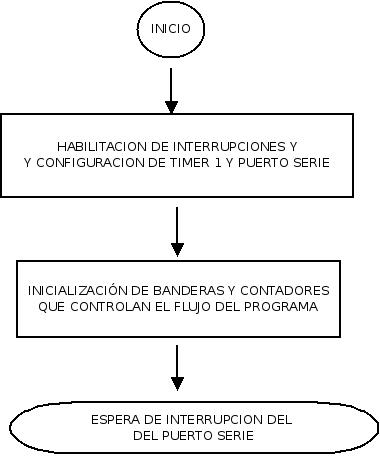
\includegraphics[width=9cm]{Imagenes/DiagFlujoAuto2.jpg}
					\caption{Diagrama de Flujo del Auto (Principal)} \label{AutoFlujo1}
				\end{figure}

				\newpage
				\begin{figure}[!htb]
					\centering
					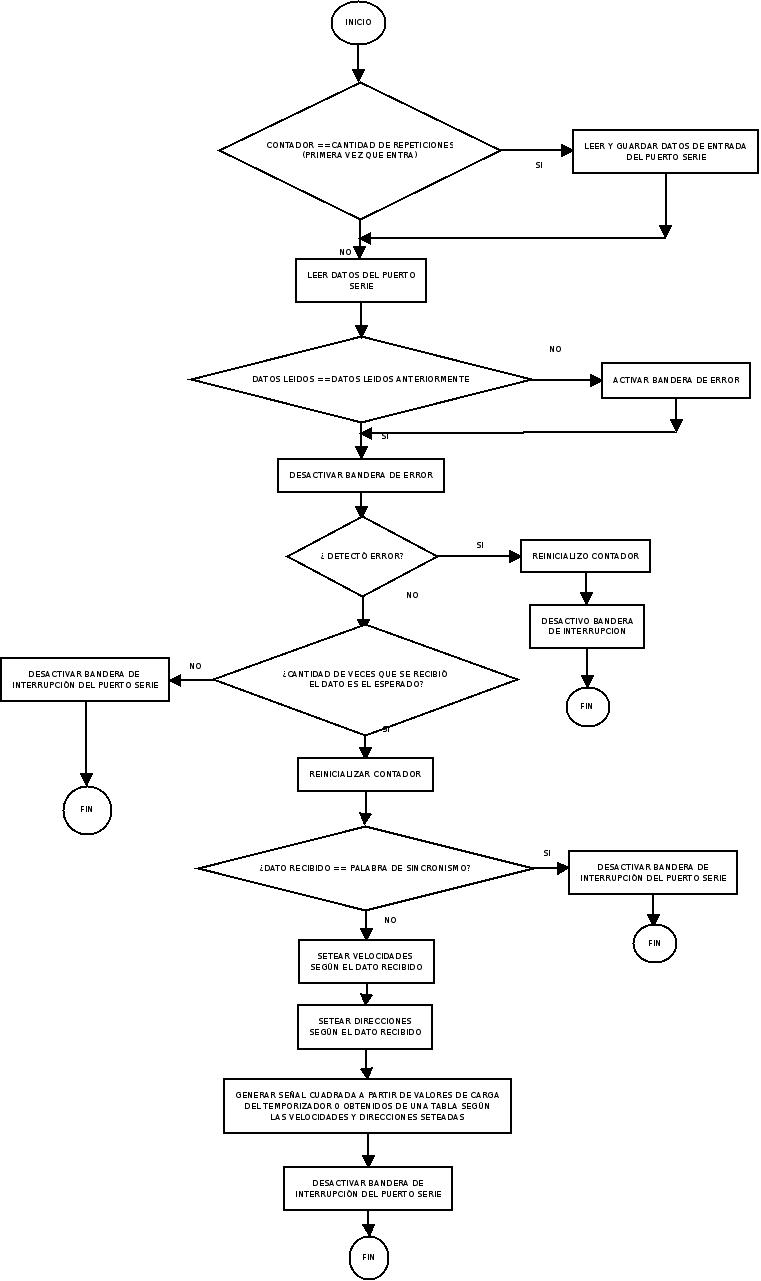
\includegraphics[width=11cm]{Imagenes/DiagFlujoAuto1.jpg}
					\caption{Diagrama de Flujo del Auto (Interrupción Puerto Serie)} \label{AutoFlujo2}
				\end{figure}

	% Negrada
	\vspace{1cm}
				\subsection{Control}
					
					\begin{figure}[!htb]
						\centering
						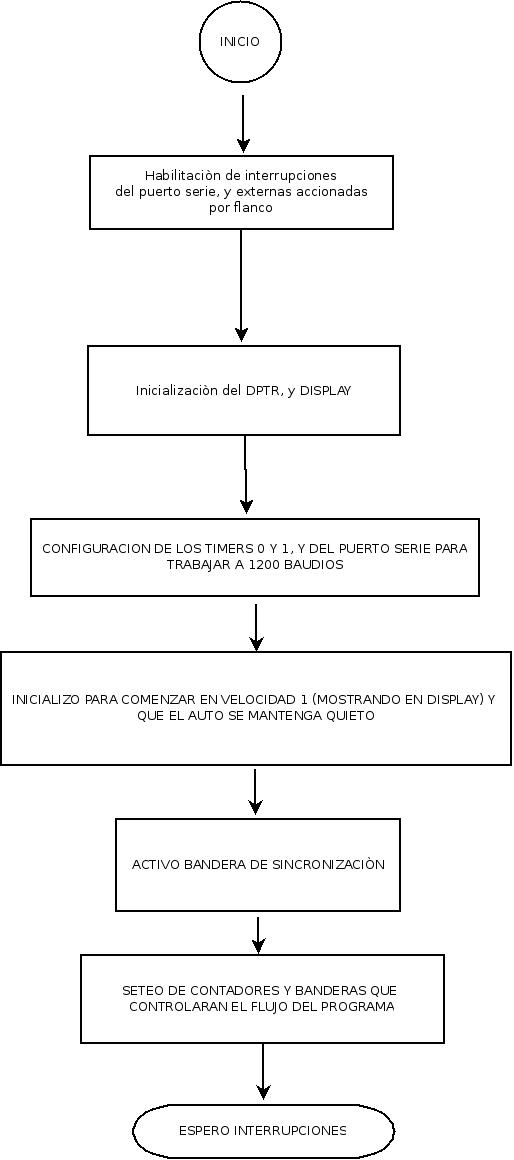
\includegraphics[width=8cm]{Imagenes/DiagFlujoControl4.jpg}
						\caption{Diagrama de Flujo del Control (Principal)} \label{ControlFlujo1}
					\end{figure}

					\newpage
					\begin{figure}[!htb]
						\centering
						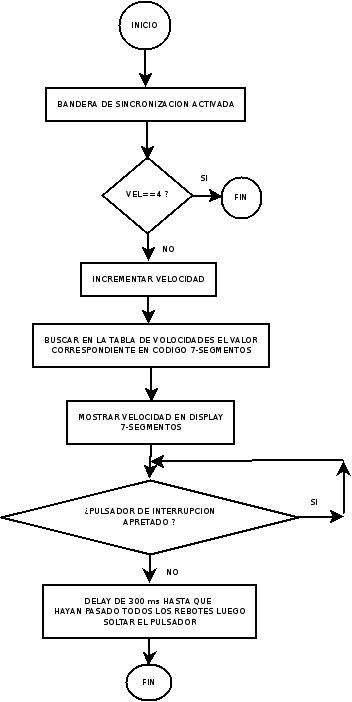
\includegraphics[width=9cm]{Imagenes/DiagFlujoControl3.jpg}
						\caption{Diagrama de Flujo del Control (Int. Externa 0)} \label{ControlFlujo2}
					\end{figure}
			
					\newpage
					\begin{figure}[!htb]
						\centering
						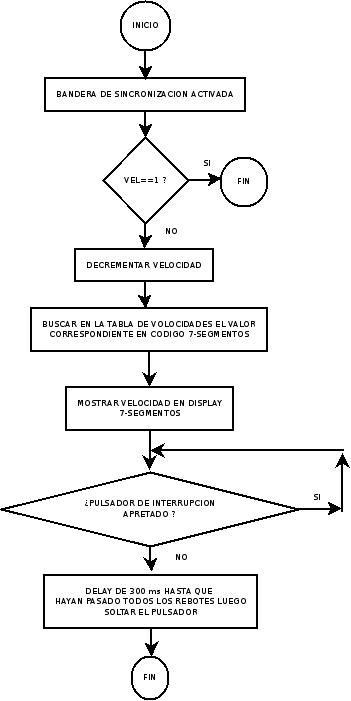
\includegraphics[width=9cm]{Imagenes/DiagFlujoControl2.jpg}
						\caption{Diagrama de Flujo del Control (Int. Externa 1)} \label{ControlFlujo3}
					\end{figure}

					\newpage
					\begin{figure}[!htb]
						\centering
						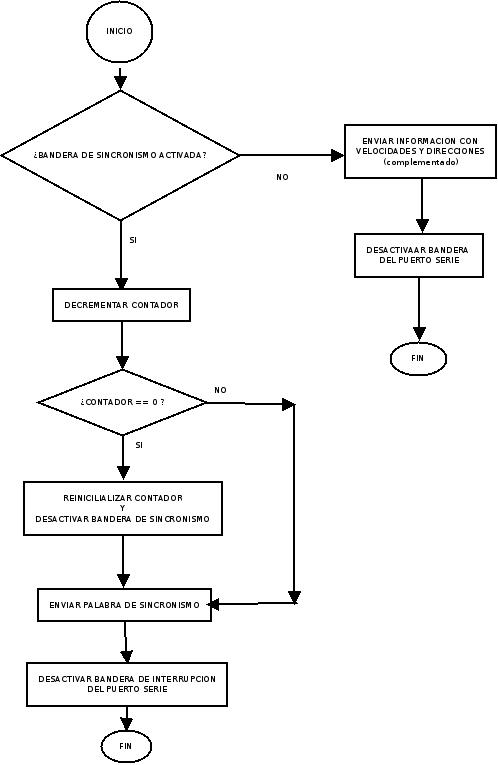
\includegraphics[width=9cm]{Imagenes/DiagFlujoControl1.jpg}
						\caption{Diagrama de Flujo del Control (Int. Puerto Serie)} \label{ControlFlujo4}
					\end{figure}
\end{document}
